% Created 2018-02-21 Wed 19:30
% Intended LaTeX compiler: pdflatex

\documentclass[twocolumn,twoside]{IEEEtran}
% \documentclass[journal,twocolumn,twoside]{IEEEtran}
% \documentclass[journal,12pt,onecolumn,draftclsnofoot,,twoside]{IEEEtran/IEEEtran}
\pdfminorversion 4 % This is so manuscript central can use it.

% \usepackage[utf8]{inputenc}
% \usepackage[T1]{fontenc}
% \usepackage{grffile}
% \usepackage{rotating}
% \usepackage[normalem]{ulem}
% \usepackage{hyperref}
% \usepackage{textcomp}
% \usepackage{capt-of}


\usepackage{graphicx}
\usepackage{cite} % Need this to get compressed citation, e.g., [4]-[7]
\usepackage{longtable}
\usepackage{wrapfig}

\usepackage{booktabs}
\usepackage{amsmath}
\usepackage{amssymb}
\usepackage[inkscapelatex=false, inkscapepath=svgsubpath]{svg}
\usepackage{subcaption}
\usepackage{xspace, dsfont}
\usepackage{mathtools}
\usepackage{multirow}
\usepackage{overpic}
\usepackage[table]{colortbl}

\usepackage[textsize=tiny,textwidth=1\marginparwidth,draft,obeyFinal]{todonotes}

\usepackage{courier} %for fixed-width, \texttt{stuff}
\newcommand{\Dm}{\ensuremath{\mathcal{D}_{-} }\xspace}
\newcommand{\U}{\ensuremath{\mathcal{U} }\xspace}
\newcommand{\DU}{\ensuremath{\Delta \mathcal{U} }\xspace}
\newcommand{\Q}{\ensuremath{\mathcal{Q} }\xspace}
\newcommand{\R}{\ensuremath{\mathcal{R} }\xspace}
\newcommand{\Hh}{\ensuremath{\mathcal{H} }\xspace}
\newcommand{\du}{\ensuremath{\Delta u }\xspace}
\newcommand{\dU}{\ensuremath{\Delta \mathcal{u} }\xspace}
\newcommand{\Gd}{\ensuremath{\bar G }\xspace}
\newcommand{\Ad}{\ensuremath{\bar A }\xspace}
\newcommand{\Bd}{\ensuremath{\bar B }\xspace}
\newcommand{\Cd}{\ensuremath{\bar C }\xspace}
\newcommand{\xd}{\ensuremath{\bar x }\xspace}
\newcommand{\Qd}{\ensuremath{\bar Q }\xspace}
\newcommand{\Rd}{\ensuremath{\bar R }\xspace}
\newcommand{\x}{\ensuremath{x }\xspace}
\newcommand{\xdss}{\ensuremath{\bar x_{ss} }\xspace}
\newcommand{\xde}{\ensuremath{\bar x_{e} }\xspace}
\newcommand{\xo}{\ensuremath{\hat x }\xspace}
\newcommand{\yr}{\ensuremath{y_{r} }\xspace}
\newcommand{\y}{\ensuremath{y} \xspace}
\newcommand{\dd}{\ensuremath{\Delta }\xspace}
\newcommand{\Gv}{\ensuremath{G_{\text{vib}}}\xspace}
% \newcommand{\ub}{\ensuremath{\bar{u} }\xspace}
% \newcommand{\ubp}{\ensuremath{\bar{u}^+ }\xspace}
% \newcommand{\ubm}{\ensuremath{\bar{u}^- }\xspace}


\begin{document}
\title{Control strategies for step tracking a piezo stage}
\author{Roger A. Braker and Lucy Y. Pao
  \thanks{The authors are with the Dept. of Electrical, Computer, and Energy Engineering at the University of Colorado, 425 UCB, Boulder, CO 80309, United States. Phone: +1 (303) 492-2360. Fax: +1 (303) 492-2758.
    R. A.  Braker (corresponding author roger.braker@colorado.edu) is a graduate student and
    L.Y. Pao (pao@colorado.edu) is the Richard \& Joy Dorf Professor.}
  \thanks{This work was supported in part by the US National Science Foundation (NSF Grant CMMI-1234980), Agilent Technologies, Inc., and the Hanse Wissenschaftskolleg in Delmenhorst, Germany.}
}

\maketitle
\begin{abstract}
  This paper considers the setpoint tracking performance of piezo nano-positioning stage subject to rate of change limitations of the control signal imposed by the power amplifier. We compare the settling-time performance of a Model Predictive Control scheme to saturated linear feedback to compensate the vibrational dynamics of the stage. In both cases, hysteresis and drift are compensated via dynamic inversion. 
\end{abstract}


\section{Introduction}\label{sec:intro}

The Atomic Force Microscope (AFM) is a nano-scale imaging instrument which acquires an image of the surface topography of a sample by mechanically interrogating it with an atomically-sharp probe.  \cite{abramovitch_tutorial_2007}. Typically, the probe is scanned across a specimen in a raster patter, sequentially acquiring pixels in an image. Although this process gives the AFM with excellent spatial resolution, the serial acquisition of pixels limits the speed of any given instrument, yielding frame rates on the order of minutes for many commercially available instruments.

While slow imaging is inconvenient for static samples, it represents a fundamental limitation in the study of dynamic specimens. Many methods have been proposed to increase AFM framerates include better mechanical design, \cite{schitter_designmodeling,kenton_threeaxis}, using advanced control methods,  \cite{butterworth_dualadaptive_2011, li_feedforward_2007, Leang_IEEECS_2009, reza_zaxis_videorate} and alternative scanning methods \cite{Mahmood_nano_2009,Tuma:2012hv,rana_spiral_2014,fleming_bridging_2010, Huang:2014dw,Hartman:2017ud}.

Our interest here is the application of Compressive Sensing to AFM, which is a newer alternative to raster scanning which has seen recent interest~\cite{oxvig_structure_2017, andersson_pao, song_video_2011}. The central idea of CS-based imaging is to leverage the redundancy present in most interesting signals such that the  number of pixels to be acquired is reduced. For good guarantees on reconstruction quality, measurements in CS-based imaging need to be randomly distributed across the specimen. Each measurement might acquire a single pixel \cite{andersson_pao} or short micro-scan \cite{braker_hardware_2018, maxwell_acc_2014}. Once a measurement is completed, the AFM probe is retracted from the sample surface, then moved in the XY plane to the next measurement location, the probe is re-engaged with the surface and the next measurement is acquired. Details of a basic implementation of this approach can be found in \cite{braker_hardware_2018}.

In this paper we are concerned with the point-to-point movement in the XY plane between measurement locations. 
Point-to-point movements by AFM is also of interest in other areas like visceolastic property mapping \cite{killgore_visceolastic_2011}.

\begin{figure*}
  \centering
  % [grid]
  \begin{overpic}[scale=1]{figures/blocks/ss_block_diagram_cropped.pdf}
    \put(63.,19){$\mathcal{F}${\raisebox{1.15ex}{$\scriptscriptstyle -1$}}$[\cdot]$}
    \put(76.4,19){$\mathcal{F}[\cdot]$}
% \includegraphics                
\end{overpic}
  \caption{The overall plant model consists of a hysteresis model $\mathcal{F}[\cdot]$,  a drift model $G_{d}$ and a vibrational model, $\Gv$. The affects of drift and hysteresis are compensated for via dynamic inversion.}
  \label{fig:ss_bd}
\end{figure*}

One of the primary constraints in setpoint tracking with our piezo stage is the current limit of the power amplifier,  which roughly translates to a slew rate limitation on the control signal.
In principle, minimizing the tracking time of such point-to-point motions is a classic time-optimal control problem. % For piezo stages which can be adequately modeled as a second-order system, we have considered robust methods to effect this \cite{braker_proximate_2017}. 
However, for stages with more complex dynamics,  including the stage in our own lab, closed-form solutions to the minimum-time problem are intractable.
% , rendering the methods presented in \cite{braker_proximate_2017} inapplicable.


An enticing alternative to explicitly handle the slew rate constraint is Model Predictive Control (MPC).
Given a discrete-time state space system $\{A,B,C,0\}$ with state $x_k$, and control input $u_k$, an MPC scheme solves, at each time step, the optimal control problem 
\begin{subequations}
\begin{align}
\min_{v}\:\:& z^T_{N}Pz_{N} + \sum_{i=0}^{N-1}z_{i}^{T}Qz_{i} + 2z^T_iSu_i + v^{T}_{i}Rv_{i} \\
 \text{s.t.} \quad z_{i+1} &= A z_{i} + B v_{i}\\
z_{0} &= x_{k}, \\
v_i  &\in \mathds{U}
\end{align}\label{eqn:optcost0}%
\end{subequations}
where $\mathds{U}$ is a convex set, $P$ solves the Discrete Algebraic Riccati Equation (DARE), $Q$ and $R$ are symmetric matrices and, together with $S$, satisfy
\begin{align}
  R &> 0 \label{eqn:schur0}\\
  Q - SR^{-1}S^T &\geq 0. \label{eqn:schur1}
\end{align}
% \begin{equation}
%   \begin{bmatrix}
%     Q & S\\S^T &R
%   \end{bmatrix} > 0.
% \end{equation}
The solution to the quadratic program (QP) \eqref{eqn:optcost0} results in a sequence of optimal controls $v_0\dots v_{N-1}$. One sets $u_k = v_0$ and repeats the process at the next time step.

Historically, one of the challenges of applying MPC to systems with fast dynamics is the computational demands imposed by solving a QP within a small sample period. However, advances in both in both hardware and algorithms have mitigated this issue. For example, \cite{Jerez_Trans_2014} shows that when $\mathds{U}$ is a simple box (i.e., a saturating constraint), sample rates of up to 1 MHz can be achieved with high-end FPGAs using an algorithm called the Fast Gradient Method (FGM). In recent work, we applied the FGM formulation of \cite{Jerez_Trans_2014} to our piezo stage and showed that, given a particular set of weighting matrices, we could improve the stabilizable region of setpoints compared to simply saturating an equivalent linear feedback \cite{braker_application_2017}.

One question which naturally arises from that study, is "how much \emph{time} is actually saved with MPC?" In essence, the stabilizable set of setpoints using saturated linear feedback can be expanded by relaxing the performance criteria.
% While we might expect this to result in a slower settling time, the question we seek to answer is \emph{how much slower}?
In other words, given a range of setpoints we wish to be able to visit, to what extent does the additional aggressiveness permitted by MPC reduce the settling time and is this reduction significant enough to warrant the additional complexity?

Additionally, we did not give any consideration to the robustness of our scheme. This is a limitation shared with other relevant applications of MPC to mechatronic systems \cite{Wills_CDC_2005, Lin_ASME_2012, rana_design_2014}. Nominally of course, MPC is a non-linear control law. However, when the solution to \eqref{eqn:optcost0} is within the interior of $\mathds{U}$, the control action is equivalent to a linear feedback law. In the situation we consider where the constraint limits the rate of change on the control, this will always be the case as the systems nears a given setpoint. Thus, within some region around any setpoint, classical ideas like gain and phase margin are directly applicable. We show in Section~\ref{sec:results} that improving these margins has a stronger influence on the experimental settle-time over a wide range of step inputs compared to a design that focuses only on increasing the aggressiveness of the control law.

A related limitation of \cite{braker_application_2017} is that we did not consider the affects of drift and hysteresis and only considered tracking a single setpoint with the stage starting at rest. When tracking a \emph{sequence} of setpoints across the range of the stage, the affects of hysteresis become much more prominent. Thus, in this paper, we employ inverse drift and hysteresis compensation. However, these inversions are not perfect, which contributes to the need for good stability margins.

The overall control structure we consider in this paper is illustrated in the block diagram in Fig. ~\ref{fig:ss_bd}. We consider the plant to be a cascaded model of hysteresis ($\mathcal{F}$),  drift ($G_d$) and vibrational dynamics ($\Gv$). Modeling these three systems are the subject of Sections \ref{sec:hyst_model}, \ref{sec:drift_model}, and \ref{sec:vib_model} respectively. Section~\ref{sec:control_setup} develops the control structure and associated closed-loop equations. Section~\ref{sec:tune} explores two schemes to design the weighting matrices and their ramifications on robustness. 

% We want to look at a few different ways of driving the stage from point to point as rapidly as possible, yet still be practical. Inspired by our past work, we focus on the experimental comparison of two methods:
% \begin{itemize}
% \item\emph{Saturated Linear state feedback (SLF)} The basic idea here to use standard linear state feedback which is saturated (on $\Delta u$) but to de-rate the design such that the closed-loop system is demonstrably stable up to a certain reference size. 
% \item\emph{Constrained Model Predictive Control (MPC)} The goal with MPC is that, instead of fully de-rating the design to account for the slew rate constraint, to directly account for the constraint as part of the control law itself. Due to limitations on the implementation, MPC must still be de-rated to some extent to be implementable, since the length of control horizon needed to achieve stabilty over the full range of the stage becomes large for an aggressive design.
% \end{itemize}

\section{Experimental Testbed}\label{sec:testbed}
The AFM in our lab consists of an Agilent 5400 which has been retrofitted with an nPoint NPXY100A piezo stage, which provides lateral movement of the sample. The NPXY100A, which is the focus of this paper, is driven by an nPoint C300. The C300 amplifies the low voltage ($\pm~10$ volts) control inputs to a high voltage signal which drives the piezo actuators and provides signal conditioning for the capacitive position sensors in the stage. Although the C300 can implement a basic PID controller, in this work we always operate the C300 in open-loop mode. Unfortunately, even in open-loop mode, signals in the C300 still run through an internal DSP, which introduces around 360 $\mu$s of delay. 

All control logic is programmed into a Xilinx Spartan-6 LX150 FPGA in a cRIO 9082 from National Instruments.
% Due to limitations in the digital to analog converter, the maximum sampling frequency is 100~kHz.
In this work we use a sampling frequency of 25~kHz, which is based on the system dynamics (see Fig.~\ref{fig:Guz2stage_frf} in Section \ref{sec:vib_model}). The sampling frequency of 25~kHz, the approximate 360~$\mu$s of delay translates to about 9 samples.

In characterizing the limitations of this system, it will be helpful to enable a direct measurement of the power amplifier current, $I_X$, of the C300. This measurement is obtained by re-routing the C300 drive signal through a low-side current sensing resistor ($0.1\Omega$) as shown in Fig.~\ref{fig:c300_meas}.
The voltage across this resistor is amplified by an op-amp circuit so that
\begin{equation}
I_{X} = \frac{1}{K_{op}R_{\text{sense}}}V_{op}
\end{equation}
where $K_{op}\approx 151$ is the gain of the operational amplifier.


\begin{figure}
    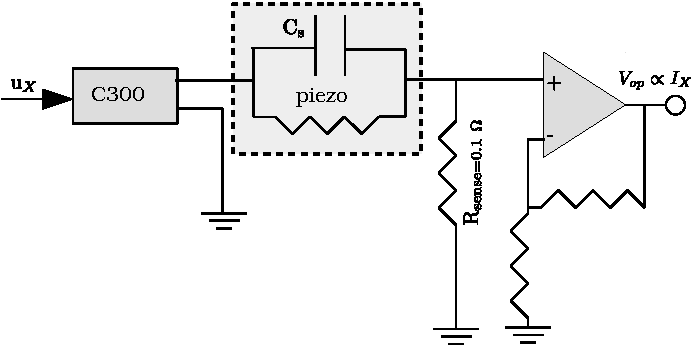
\includegraphics[width=1\columnwidth]{figures/blocks/c300_measurement_cropped.pdf}
    \caption{Schematic of the augmented current measurement used in characterizing the C300.}
    \label{fig:c300_meas}
  % \end{minipage}
\end{figure}
\section{System Modeling}

To keep the discussion manageable, we will concentrate the discussion to the $X$-direction. We model the overall plant for the $X$-direction as three cascaded systems: $\mathcal{F}$ which models the hysteresis of the piezo, a drift model $G_d$ and a vibrational model $\Gv$. This cascaded structure is shown in Fig.~\ref{fig:ss_bd}. In general, the effects of hysteresis are most noticeable when moving across wide ranges. Thus, by using relatively small input signals, the drift and vibrational dynamics can be identified separately from the hysteresis. Here, we model both $\Gv$ and $G_d$ as linear, time-invariant discrete-time systems. The dynamics of drift are predominantly low frequency while vibrational aspects on the other hand are fast by comparison, which allows the two systems to be easily separated in the identification.
 Modeling these three components is the subject of the next three subsections.


\subsection{Modeling \Gv}\label{sec:vib_model}
To obtain an experimental frequency response of $\Gv$, we use a stepped-sines method (single frequency at a time). The amplitude of the driving sinusoid is chosen to be small enough that the effects of hysteresis are minimized. After the system reaches steady-state, the input and output signals are demodulated into their first (complex) Fourier coefficients, the ratio of which yields the frequency response at that frequency. Fig.~\ref{fig:Guz2stage_frf} shows the resulting experimental FRF as the solid red curve.

\begin{figure}
  \centering
  \includesvg[width=01\linewidth]{figures/G_uz2stage_Eres.svg}
  \caption{The solid red curve (left axis) is the frequency response from control input to stage position output in the $X$ direction. The dashed-black curve is the model.}
  \label{fig:Guz2stage_frf}
\end{figure}

Obtaining a parametric model of $\Gv$ for control design involves two steps. We obtain a preliminary model using an Eigenspace Realization Algorithm (ERA) \cite{Jacques_sysidfrf}. In general, the ERA does not produce a model with poles at $z=0$, which is what we need in order to model the delay. Thus, the delay in the frequency response is divided out of the FRF before passing it to the ERA algorithm.

The second step uses the model generated by the ERA as the initial guess to a non-linear least squares problem \cite{sidman_parametric_1991} which minimizes the ratio of the logarithm of the experimental frequency response to that of the model. Though Sidman et al. develop the idea for continuous time models, their strategy is easily adapted to fit a discrete time model. In this scenario, the optimization is given by
\begin{align}
\min_{\theta} \sum_{i=1}^M| \log(G(e^{j\omega_iT_s})) - \log(\hat{G}(e^{j\omega_iT_s}|\theta))|^2
\label{eqn:logfit}
\end{align}
where $\omega_i$ is each frequency in the experimental frequency response and $\hat{G}(e^{j\omega_iT_s}|\theta)$ is the model parametrized by the vector $\theta$. The model $\hat{G}(z|\theta)$ is composed of first and second-order factors
\begin{equation}
  \hat{G}(z|\theta) =K \frac{\prod_{i=0}^{n_{rz}-1} (z-b^r_i) \prod_{j=0}^{2n_{cz}-1}(z^2 +b^c_{2j}z + b^c_{2j+1})}
  { \prod_{l=0}^{n_{rp}-1}(z-a^r_l) \prod_{m=0}^{2n_{cp}-1}(z^2 +a^c_{2m}z + a^c_{2m+1})}z^{-p} \label{eqn:mode_struc}
\end{equation}
so that
% \todo{Do you think this is too much detail here?}
\begin{equation}
\theta = [b^r_0\dots b^r_{n_{rz}}, b^c_{0}\dots b^c_{2n_{cz}-1}, a^r_0\dots a^r_{n_{rp}}, a^c_{0}\dots a^c_{2n_{cp}-1}, k, p].
\end{equation}
Due to the logarithms in \eqref{eqn:logfit} and the multiplicative structure \eqref{eqn:mode_struc}, the Jacobian of $\log(\hat{G}(z|\theta))$ is surprisingly easy to calculate. Details can be found in \cite{sidman_parametric_1991}, though some modifications are required for the discrete-time case.

The model structure \eqref{eqn:mode_struc} includes a fractional delay $z^{-p}$. This allows us to include the delay as a term in the decision variable and obviates the need to optimize over integers. This is further beneficial because we are not guaranteed that the latency from input to output is an exact integer and allowing a fractional delay helps the optimization to more accurately match the phase. In the final model, we round $p$ to the nearest integer. In this work, we do not model the modes above 1100~Hz. Thus, the optimization \eqref{eqn:logfit} is only done over frequency up to 1100~Hz. The final pole and zero locations for $\Gv$ are listed in Table \ref{tab:pzgvib}.

\begin{table}
  \centering
  \caption{Zero and pole locations of $\Gv$. }
  \label{tab:pzgvib}
  \begin{tabular}{cc}
    pole & zero\\
    0.848155$\pm$0.187900 & 0.964821 $\pm$ 0.250813\\ 
    0.962030$\pm$0.259730 & 0.992956 $\pm$ 0.093824\\ 
    0.972209$\pm$0.213448 & 0.975116 $\pm$ 0.209867\\ 
    0.978579$\pm$0.163808 & --\\ 
    0.993712$\pm$0.091498 & --\\ 
    0.917539 & 0.505483 \\ 
    (9) 0.0 & 0.822878 \\ 
  \end{tabular}
\end{table}


\subsection{Drift Modeling}\label{sec:drift_model}

% It is very common in the literature to fit a drift model to a single step input \cite{liu_creep_2013, croft_creep_1999}. This does not seem to be sufficient.

% It has been noted before in the literature that the rate of the creep affect itself is hysteretic \cite{Jung_open_loop_2000}, which I think in this context would imply that the real pole-zero pairs of $G_{drift}$ shift depending on the control history.


We model drift as the strictly proper transfer function
\begin{equation}
G_d(z|\theta) = \theta_5\frac{(z-\theta_1)(z-\theta_2)}{(z-\theta_3)(z-\theta_4)}.
\end{equation}
We give the stage a step input with relatively small amplitude (to minimize the effects of hysteresis). The stage response is shown as the solid-blue curve in Fig.~\ref{fig:drift_fit} while the simulated response of the vibrational model is shown as the dotted-black curve. The drift in the stage is evident in the slow increase of stage position after the vibrational dynamics have decayed. 

\begin{figure}
  \includesvg[width=1\linewidth]{figures/drift_fit.svg}
  \caption{The stage is given a step input (dash-dotted blue) with an amplitude of 0.15 volts, which results in the solid blue output trajectory. The response of the combined $\Gv$ and $G_{d}$ models is shown as the dashed red, while the vibrational model alone is the dotted black curve.}
  \label{fig:drift_fit}
\end{figure}

Let $\mathcal{Y}_{exp}$ be the step response data collected from the stage and  $\mathcal{Y}_{vib}$ be the response of the model $\Gv$ to the same input. The goal then is to solve the non-linear least squares problem
% \todo{I think this is a bit awkward}
\begin{equation}
  \min_{\theta}|| g_d(k|\theta)*\mathcal{Y}_{vib} - \mathcal{Y}_{exp}||_2
  \label{eqn:fit_drift_cost}
\end{equation}
where $g_d(k|\theta)$ is the impulse response of $G_d(z|\theta)$, '$*$' represents the convolution operator and  $\theta$ is the vector of parameters. To the extent that $\Gv$ accurately models the vibrational dynamics, the inclusion of $\mathcal{Y}_{vib}$ in \eqref{eqn:fit_drift_cost} effectively nullifies the vibrational aspects in the optimization. This is possible because, since we have a SISO system, $\Gv$ and $G_d$ commute. 
The non-linear optimization problem \eqref{eqn:fit_drift_cost} is solved with MATLAB's \texttt{lsqnonlin} and results in the red curve in Fig.~\ref{fig:drift_fit} which shows the simulated step response of $G_d\Gv$. 


\subsection{Hysteresis Modeling}\label{sec:hyst_model}
In typical raster scanning applications, hysteresis manifests as a bowing of the trajectory as the stage tries to track the linear ramps in a triangle wave (see, e.g., Fig. 3 of \cite{Leang_IEEECS_2009}). To motivate the need for hysteresis compensation in a step tracking application, consider Fig. \ref{fig:hyst_resp_dem}, which shows an input signal of various filtered steps applied open-loop to the stage. The solid black curve is the stage response, while the dotted-black curve is the input (scaled by the nominal DC-gain of $G_d\Gv$), which shows good agreement for the first step, but much worse agreement with the later steps, particularly those with large amplitudes. Effectively, the gain of the system depends on the control history, since for the same steady state value of control, the steady state value of the stage changes.

There are many models for hysteresis \cite{croft_creep_1999, rakotondrabe_bouc_2011, Lui_hysteresis_2013}. Here, we opt for simplicity (and by proxy, fast computation) and use the Modified Prandtl-Ishlinksi Hysteresis model developed in \cite{kuhnen_modeling_2003}. This hysteresis model is composed of a linear combination of saturation operators cascaded with a linear combination of classic hysteretic play\footnote{The term ``play'' is derived from the operator's use in modeling mechanical slop.} operators. This cascaded structure is illustrated in Fig.~\ref{fig:ss_bd}. The overall input-output relationship of the modified hysteresis operator $\mathcal{F}[\cdot]$ is
\begin{equation}
  \mathcal{F}(u_X) = w_s^T\mathbf{S}\left[w_H^T \mathbf{H}[u_X, z]\right]
\end{equation}
where $\mathbf{S}$ and $\mathbf{H}$ are vectors of elementary saturation and play operators respectively, and
where $w_s$ and $w_H$ are vectors of weights. The input-output relationship of the $i$th elementary saturation operator with associated threshold $d_s^i$ is defined as
\begin{align}
  \mu_k=
  S^i(\xi_k| d_S^i) &=
  \begin{cases}
    \max\{\xi_k - d_S^i, 0\} & d_S^i >0\\
    \xi_k & d_S^i = 0\\
    \min\{\xi_k-d_S^i, 0\},  & d_S^i<0.
  \end{cases}
\end{align}
for an input $\xi_k$ and output $\mu_k$. 

In contrast, the elementary play operators have memory. The $i$th elementary play operator with associated threshold $d_H^i$, output $\xi_k^i$ and input $\nu_k$ is defined by the recursive relationship
\begin{align}
  \xi_k &=
  H^i(\nu_k|\: d_H^i) =
  \max\{\xi^i_{k-1}-d_H^i, \min\{\xi^i_{k-1} + d_H^i, \nu_k\} \}
\end{align}
If the thresholds $d_H^i$ and $d_S^i$ are pre-defined, \cite{kuhnen_modeling_2003} shows that it is possible to fit the weights $w_S$ and $w_H$ as the solution to a quadratic program. The resulting fit with 7 saturation operators and 7 hysteresis operators is shown in Fig.~\ref{fig:hyst_resp_dem} as the dashed red curve (which also includes the drift and vibrational models). As the inset in that figure shows, it is possible to improve on the fit. One common alternative to cascading the drift and hysteresis models is to put them in parallel with each other \cite{mokaberi_compensation_2008, Krejci_inverse_2001}. While this does indeed lead to a smaller residual, it gives worse closed-loop performance than the present method.

\begin{figure}
  \includesvg[width=1\linewidth]{figures/hyst_response_ol.svg}
  \caption{The stage is driven by a sequence of filtered step inputs shown in the dotted black curve. The resulting stage response is the solid black curve, which shows good agreement, e.g., at the first step, but much worse agreement for larger steady state values. The dashed red curve is the response of the overall combined model of $\Gv$, $G_{d}$, and the complex hysteresis model $\mathcal{F}$.}
  \label{fig:hyst_resp_dem}
\end{figure}


\subsection{Power Amplifier Characterization and Limitations}\label{sec:powcharct}
\begin{figure}[htbp]
\centering
\includesvg[width=1\linewidth]{figures/G_pow_and_current.svg}
\caption{
  Frequency responses for the power amplifier. The solid red curve is the transfer function from the low voltage command to the high voltage output $G_{V_X, u_X}$. The solid blue curve transfer function from high voltage output to current output. The solid black is the transfer function from low voltage control to power amplifier output current $G_{V_X, u_X}$, which is upper-bounded by the dotted-back curve representing $\tilde G_{I_X, u_x}$, a pure discrete derivative.}
\label{fig:powTF}
\end{figure}

The high voltage output of the C300 is current limited to 100 mA. The solid black curve in Figure~\ref{fig:powTF} shows the transfer function from the low voltage input of the C300 to current flowing through the stage, $G_{I_X,u_X}$. Because the piezo actuators are highly capacitive, at frequencies below about 600~Hz, $G_{I_X,u_x}$ looks like a pure derivative.
Thus, we can factor $G_{I_X,u_X}$ as
\begin{align}
  I_{X}(z) &= G_{I_X,u_X} u_X(z)\label{eqn:Gix_statebound}\\
          & = (z-1) G_o u_X(z)\\
          & = G_o(z) \Delta u_X(z) \label{eqn:Gostatebound}
\end{align}
Ideally, one would enforce the current limit via a state-like constraint using \eqref{eqn:Gix_statebound} and a parametric model of $G_{I_X,u_X}$.
Although it is likely possible to solve such a problem with a high-end FPGA~\cite{Jerez_Trans_2014}, it is not possible to solve that problem on our hardware. Instead, we would like to approximate $G_o$ as a constant, which will lead to a box constraint on $\Delta u_X$. Thus, we need a bound $(\Delta u_k)_{\text{max}}$ such that
\begin{equation}
  |\Delta u_X(k)| < (\Delta u_X)_{\text{max}} \implies |I_{\text{pow}}| < I_{\text{max}}.\label{eqn:du_bound0}
\end{equation}
It is straightforward to show such a bound is given by 
\begin{equation}
\Delta u_X(k))_{\text{max}} = \frac{I_{\text{max}}}{||g_o||_1}
\end{equation}
where $g_o$ is the impulse response of $G_o(z)$ and $||g_o||_1 = \sum_{k=0}^{\infty}|g_o(k)|$. The frequency response of this bound is shown in Fig. \ref{fig:powTF} as the dotted-black curve. In practice, we find that this bound is overly conservative. An alternative is to choose
\begin{equation}
(\Delta u)_{\text{max}} = ||G_o(z)||_{\infty}\approx 0.1980, \label{eqn:duHinf}
\end{equation}
which is the dashed-black curve in Fig.~\ref{fig:powTF}. Although \eqref{eqn:duHinf} is only sufficient to guarantee \eqref{eqn:du_bound0} for sinusoidal inputs, in practice we find that enforcing \eqref{eqn:duHinf} does lead to the current staying under 100~mA.

% Notably, this bound is conservative, since for higher frequencies a pure derivative overestimates the amount of actual current draw. Ideally, we would use a parametric model of \(G_{I_{X},u_{X}}\) and enforce a constraint on the output of that model. However, such an approach renders the constraint set for $u_X$ complex and is it not feasible to solve that problem using the fast gradient method. In our experimental implementations, we will enforce \eqref{eqn:du_limit}.
% However, in Section~\ref{sec:time_save_analysis} we will consider how much performance is given up through this method via a simulation study. 

Finally, the slew rate limit used in the MPC/linear feedback controller must be discounted from \eqref{eqn:duHinf} to account for the inverse inverse drift compensator. This adjustment for the inverse drift operator follows essentially the same argument as above. We have
\begin{equation}
  (\Delta u)_{\text{max}} \leq \frac{(\Delta u_X)_{\text{max}}}{||G^{-1}_d(z)||_{\infty}} \approx 0.167 \label{eqn:du_discount}
\end{equation}
% \todo{should I say something about hysteresis inversion in the context}
\section{Control Setup}\label{sec:control_setup}
The constraint \eqref{eqn:du_discount} can be remodeled as a pure saturating constraint if we work with an incremental form of \(\Gv\) which has as its input \({\Delta u_k\coloneqq u_k-u_{k-1}}\), rather than \(u_k\). This is attractive because it not only allows us to directly penalize the rate of change in the optimal control problem but also renders the constraint \eqref{eqn:du_discount} as a box constraint on $\Delta u$, enabling the use of the computationally attractive Fast Gradient Method. Details on the form of the FGM we use can be found in \cite{Jerez_Trans_2014, jerez_embedded_2013} while specifics about our implementation are discussed in \cite{braker_application_2017}
% \todo{Do you think I need to talk more about the FGM?}
% Putting a hard limit on $\Delta u$ in the linear feedback case is also simplified.
\subsection{The Incremental Form}\label{sec:incremental}
To develop the required incremental form, we augment the dynamics of \(\Gv=\{A,B,C,0\}\) with a state \(\x_{\text{u}}(k)\) such that
\begin{equation*}
  \x_{u_k} = u_{k-1}.
\end{equation*}
It follows that
\begin{subequations}
\begin{align}
  % \begin{bmatrix}\x_{k+1}\\\x_{u_{k+1}}\end{bmatrix}
  \xd_{k+1}
  &=
    \begin{bmatrix}
      A & B\\ 0 & 1
    \end{bmatrix}
                  \xd_k
    % \begin{bmatrix}\x_k\\\x_{u_k}\end{bmatrix}
    +
    \begin{bmatrix}
      B\\1
    \end{bmatrix}
  \Delta u_k \label{eqn:deltadyn} \\
  \y_k & = \begin{bmatrix}C & 0\end{bmatrix}\xd_k\\
                              % \begin{bmatrix}\x_k\\\x_{u_k}\end{bmatrix}\\
    \xd_k& \coloneqq
    \begin{bmatrix}\x_k\\\x_{u_k} \end{bmatrix}
  % \xd(0) & = \begin{bmatrix}\x(0)\\u(-1)\end{bmatrix}. \label{eqn:x0_aug}
\end{align}\label{eqn:ssdelta}%
\end{subequations}
We call this system \(\Gd = \{\Ad, \Bd, \Cd, 0\}\), which has \({\bar{n}_s=22}\) states, 9 of which model delay.
To solve the setpoint tracking problem, we work in the error
coordinates of \(\Gd\).
For a constant reference \(r_{ss}\), in steady state we have \({\du_{ss}=0}\) and \({\xdss =N_{\xd}r_{ss}}\) where \({N_{\xd}\in\mathds{R}^{\bar{n}}}\) is found by solving
\begin{align}
  \begin{bmatrix}N_{\xd} \\ N_u\end{bmatrix} &=
\begin{bmatrix}I-\Ad & -\Bd\\\Cd & 0\end{bmatrix}^{-1}\begin{bmatrix}0\\ I\\\end{bmatrix}\label{eqn:nxnu},
\end{align}
which, due to the augmented pole at $z=1$, will give \(N_u\equiv 0\). 
The error state, \({\xd_{e_k}=\xd_k - \xdss}\) has dynamics
\begin{align}
  \xd_{e_{k+1}} & = \Ad\xd_k + \Bd\dd u_k - \xdss \nonumber\\
            & = \Ad \xd_{e_k}   + \Bd \dd u_k\nonumber
\end{align}
              because $\xdss$ is in the nullspace of $(I - \Ad)$.
              
\subsection{Observer Design}\label{sec:dist_est}
To achieve zero-offset tracking (to constant disturbances), we employ the disturbance estimator outlined in \cite{maeder_offset-free_2007}. The disturbance dynamics are modeled as a pure integrating output disturbance. The estimator dynamics are then given by
\begin{align}
  \begin{bmatrix} \hat{\x}_{k+1}\\ \hat{d}_{k+1} \end{bmatrix}
  &= A_m
  \begin{bmatrix} \hat{\x}_{k}\\ \hat{d}_k\end{bmatrix}
    + B_m u_k + L_m(y_k - \hat y_k) \label{eqn:obsdyn}\\
  \hat y_k &= C_m\begin{bmatrix} \hat{\x}_k\label{eqn:yhat}\\
    \hat{d}_k \end{bmatrix}
\end{align}
where $\hat{x}$ is our estimate of $x_k$ (not $\bar{x}_k$), $\hat{d}_k$ is the disturbance estimate, and 
\begin{align}
  A_m& = \begin{bmatrix}
    A & B_d \\ 0 & I
  \end{bmatrix},\:
  B_m =
  \begin{bmatrix}
    B \\ 0
  \end{bmatrix} \\
  C_m &= 
    \begin{bmatrix}
    C \\ C_d
  \end{bmatrix},\:\:\:\:\:\:\:\:\;
  L_m = \begin{bmatrix} L_x\\L_d \end{bmatrix} \label{eqn:CmLm}
\end{align}
It is shown in \cite{maeder_offset-free_2007} that the gains $L_x$ and $L_d$ may be designed separately such that the closed-loop poles $A_m - L_mC_m$ are the same as $\sigma(A-L_xC)\cup \sigma(A_d-L_dC_d)$.
We set $L_x$ equal to the steady state solution of the discrete LQR problem applied to the dual of $G$, where $Q = Q_w + \alpha BB^T$ and $\alpha$ is a turning parameter. We design $L_d$ such that the disturbance pole is placed at $z=0.8$.

To achieve zero offset tracking, disturbance estimators re-compute the steady-state target $\x_{ss}$ at each time-step. For an output disturbance model ($B_d=0$ and $C_d=I$), this simply means that the reference is adjusted by subtracting $\hat d_k$. In other words, at each time step, we need to compute
\begin{equation}
  \bar{x}_{e} =
  \begin{bmatrix}\hat{x}_k\\x_{u_k}
  \end{bmatrix}
  - N_{\bar{x}}(r_k - \hat{d}_k).
\end{equation}
This is slightly simpler than the case for an input disturbance model ($C_d=0$ and $B_d\neq0$), which involves an additional vector-scalar multiplication and an additional vector-vector addition (see (21) in \cite{maeder_offset-free_2007}). It is shown in \cite{maeder_offset-free_2007} that output disturbance and input disturbance estimators are equivalent provided 1 is not an eigenvalue of $A$, which is the case here, because we do not estimate the state $x_u$. Thus, due to the computational savings, we use the output disturbance formulation. 
\subsection{Closed-Loop Equations}
Let us derive the closed loop equations for the block diagram of Fig.~\ref{fig:ss_bd} with the drift and hysteresis operators set to the identity and with the controller given by a partitioned feedback gain ${K = [K_x\: K_u]}$. Similarly, the observer gain is partitioned as in \eqref{eqn:CmLm}.
In closed-loop we do not estimate $\x_u$, because it is perfectly known and we do not compute the state-feedback portion of the control with $\hat d$ because the disturbance is uncontrollable from $u_k$.  
From~\eqref{eqn:ssdelta}, \eqref{eqn:obsdyn} and \eqref{eqn:yhat} we have
\begin{align}
  \hat{\x}_{k+1} &= A \hat{x}_k + Bu_k + L_x(y - \hat{y})\label{eqn:xhat}\\
  \hat{d}_{k+1}  &= \hat{d}_k  + L_d (y - \hat{y}) \label{eqn:dhat}\\
  x_{u_{k+1}}     &= x_{u_k}  + \Delta{u}_k,\label{eqn:xu}
\end{align}
where $y_k$ is the plant output. The control increment $\Delta u_k$ and control $u_k$ are given by
\begin{align}
  \Delta u_k &= -\begin{bmatrix}
    K_x & K_u
  \end{bmatrix}
  \begin{bmatrix}
    \hat{\x} \\ x_u
  \end{bmatrix}
  +
               \bar{N}(r_k - \hat{d}_k).\label{eqn:deltau}\\
  u_k &= \Delta u_k + x_{u_k}\label{eqn:uk}.
\end{align}
In \eqref{eqn:deltau}, $\bar{N}\triangleq KN_{\bar{x}}$ is the feedforward control gain, where $N_{\bar{x}}$ is defined by \eqref{eqn:nxnu}.
We can write \eqref{eqn:xhat}-\eqref{eqn:uk} as the combined state space system
\begin{align}
\tilde{\x}_{k+1} &= \tilde{A}\tilde{\x}_k + \tilde{L}y_k + \tilde{B}\bar{N}r_k\label{eqn:cntrldyn}\\
u_k &= -\tilde{K}\tilde{\x}_k + \bar{N} r_k \label{eqn:ukx}
\end{align}
where
\begin{align*}
  \tilde{A} &= \begin{bmatrix}
    A-BK_x-L_xC & B(1-K_u) & -B\bar{N} - L_xC_d\\
    -K_x        & 1-K_u    & -\bar{N} \\
    -L_dC      & 0        & 1-L_dC_d
  \end{bmatrix}\\
  \tilde{L} &= \begin{bmatrix} L_x \\ 0 \\ L_d  \end{bmatrix},\:\:
  \tilde{B} = \begin{bmatrix} B \\ 1 \\0\end{bmatrix},\:\:
  \tilde{x}_k = \begin{bmatrix} \hat{x}_k \\ x_{u_k} \\ \hat{d}_k\end{bmatrix},\\
  \tilde{K} &= \begin{bmatrix}K_x & K_u-1 & \bar{N}\end{bmatrix},\\
\end{align*}
Taking the $z$ transform of \eqref{eqn:cntrldyn} and \eqref{eqn:ukx}, we obtain
\begin{align}
  u(z) =&  \bar{N}(1-\tilde{K}(zI-\tilde{A})^{-1}\tilde{B})r(z) \label{eqn:uz}\\
       & -\tilde{K}(zI - \tilde{A})^{-1}\tilde{L}y(z).\nonumber
\end{align}
If $G(z)$ (which need not be the same as our model $\Gv$) is the transfer function of the plant, then z-transform of the output $y$ subject to an output disturbance $d$ and control input $u$ is $y(z) = G(z)u(z) + d(z)$. Combining this expression with \eqref{eqn:uz} we obtain 
\begin{align}
  y(z) &= \frac{G(z)\bar{N}(1-D_2(z))}{1 + G(z)D_1(z)} r(z) + \frac{1}{1 + G(z)D_1(z)}d(z)\label{eqn:cltf}
\end{align}
where
\begin{align}
  D_1(z) &= \tilde{K}(zI -\tilde{A})^{-1}\tilde{L}\\
  D_2(z) &= \tilde{K}(zI -\tilde{A})^{-1}\tilde{B}.
\end{align}
Thus, the loop gain is given by $L(z) = G(z)D_1(z)$ and we define the sensitivity function $\mathcal{S}(z)\triangleq (1+L(z))^{-1}$. The closed-loop poles are the transmission zeros of $1+L(z)$ and which are the union of the controller poles and observer poles, which can be seen through the separation principle or manipulation of the matrix pencil describing the transmission zeros. Moreover, in the first term of \eqref{eqn:cltf}, the observer poles are canceled by the transmission zeros of $(1-D_2(z))$. Of course, these properties only hold when the observer is a perfect model of the plant. 

The advantage in representing the closed-loop dynamics as \eqref{eqn:cltf} is that it exposes cleanly how to analyze the robustness of our designs. Due to hysteresis, the gain margin is of particular importance. 


% \begin{figure}
%   \includesvg[width=1\linewidth]{figures/obs_cl.svg}
%   \caption{(black) open-loop plant pole (x) and zero(circle) locations. (red x) closed-loop observer pole locations.}
%   \label{fig:obs_cl}
% \end{figure}


\section{Control Designs}\label{sec:tune}
We consider two methods, Model Predictive Control(MPC) and Saturated Linear Feedback (SLF).
\begin{itemize}
\item\emph{Saturated Linear state feedback (SLF)} The basic idea here to use standard linear state feedback which is saturated (on $\Delta u$) but to de-rate the design such that the closed-loop system is stable up to a certain reference size. 
\item\emph{Constrained Model Predictive Control (MPC)} The goal with MPC is that, instead of fully de-rating the design to account for the slew rate constraint, to directly account for the constraint as part of the control law itself. Due to limitations on the implementation, MPC must still be de-rated to some extent to be implementable, since the length of control horizon needed to achieve stabilty over the full range of the stage becomes large for an overly aggressive design.
\end{itemize}

Both the MPC and linear state feedback controllers can be described by the optimization
\begin{align}
\min_{v}\:\:& z^T_{N}Pz_{N} + \sum_{i=0}^{N-1}z_{i}^{T}Qz_{i} + 2z^T_iSv_i + v^{T}_{i}Rv_{i} \label{eqn:optcost}\\
  % \text{s.t.}&\nonumber\\
  \text{s.t.}\:\:  z_{i+1} =& \Ad z_{i} + \Bd v_{i}\\
z_{0} =& [\hat{x}^T_{k}, x^T_{u_k}]^T - N_{\bar{x}}(r_k-\hat{d}_k)\\
|v_i | \leq& (\Delta u)_{\text{max}}.\label{eqn:cntrl_constraint}
\end{align}
where $Q$ and $R$ are symmetric matrices and the matrices $Q,R,S$ satisfy \eqref{eqn:schur0} and \eqref{eqn:schur1}.
% \begin{align}
%   R &> 0\nonumber\\
%   Q - SR^{-1}S^T &\geq 0. \label{eqn:schur1}
% \end{align}
The terminal cost $P$ is the solution of the DARE. The solution of \eqref{eqn:optcost} results in a sequence of $N$ optimal controls, $\{v_i\}_{i=0}^{N-1}$. In the case of MPC, one sets $\Delta u_k = v_0$ and discards the remaining elements. The process is repeated at the next time step. Note that in the case of MPC, the saturator in Fig.~\ref{fig:ss_bd} is superfluous because the optimal control satisfies the constraints by design.

In the case of linear feedback, $N=1$ and we eliminate the constraint on the control \eqref{eqn:cntrl_constraint} and thus the optimal control is simply $-Kx_k$, where
\begin{equation}
  K = (\Bd^TP\Bd + R)^{-1}(\Bd^TP\Ad + S^T).
\end{equation}

The motivation for MPC here is that we hope that by directly accounting for the constraints, additional performance can be obtained. There are two perspectives one might take here. First, by directly accounting for the constraints, we should be able to use a more aggressive control (smaller $\gamma$) while maintaining stability compared to SLF.
We will show that in simulation, this idea does indeed lead to a significantly decreased settling time. However, the desire to decrease $\gamma$ must be tempered by its affect on both robustness and disturbance rejection, because these things are a metric for how the control will perform in practice. Unfortunately, we will see that decreasing $\gamma$ tends to degrade both properties for the weighting matrices we consider. 

Alternatively, one could use the same $\gamma$ for both the MPC design and SLF design (which implies, roughly,  the same set of disturbance rejection and robustness properties) and hope that the direct handling of constraints improves performance. This is the perspective taken, e.g., in \cite{Wills_CDC_2005}. While this will indeed be the case for certain sizes of setpoints (e.g., setpoints which are near the stability boundary for SLF), we will see that the difference between MPC and SLF is marginal for the majority of the movement range.

% \subsection{The ``it doesn't work'' argument}
% This needs to essentially say: we consider three methods (1) pz-cancell, (2) constant zeta (3) constant sigma. None of these three provide enough motivation for MPC.


\subsection{Control Weight Selection}
Let $Q = FF^T$ for some vector $F\in\mathds{R}^{\bar{n}_s}$, $S=F$, and $R=1+\gamma$ where $\gamma$ is a scalar parameter. Consider the fictitious output
\begin{equation}
  \eta_k = F^T\xd_k + v_k. \label{eqn:fictout}
\end{equation}
Then running cost portion of \eqref{eqn:optcost} can be written as
\begin{equation}
   \sum_{i=0}^{N-1} \eta_i^T\eta_i + \gamma v_i^T v_i.
    % &= \sum_{i=0}^{N-1} \hat{x_i}^TQ\hat{x_i} + 2x_i^TSu_i + u_i^T(R_o+\gamma)u_i
\end{equation}
As the control weight $\gamma$ becomes small, the closed-loop poles of the unconstrained LQR
will move to the zeros of $\{A, B, F^T, 1\}$ (when the solution is within the constraint set defined by \eqref{eqn:cntrl_constraint}). This is illustrated in Fig.~\ref{fig:lqr_locus}. One can usually take $\gamma$ to be small enough while still honoring \eqref{eqn:schur1}  that the difference between the desired pole location and its actual location is negligible. The direct feedthrough in \eqref{eqn:fictout} results in the cross-weighting term $S$ and is necessary if we wish to endow the fictitious system with $\bar{n}_s$ zeros in order to place all $\bar{n}_s$ poles.

Through elementary block row and column operations, it is straightforward to show that the zeros of
$\{A, B, F^T, 1\}$ are the same as the solutions of the generalized eigenvalue problem
\begin{equation}
  \begin{bmatrix}
    (A - BF^T) & 0\\
    0 & 1
  \end{bmatrix} - \begin{bmatrix}zI & 0\\0 & 0\end{bmatrix} = 0.
\end{equation}
Thus, one may find $F$ via standard pole placement techniques.

\begin{figure*}
  % \begin{minipage}{0.48\textwidth} 
    \begin{subfigure}{0.48\textwidth}
  \includesvg[width=1\textwidth]{figures/lqr_locus_constsig_0p9.svg}
  % \caption{Root locus for $R_o + \gamma$. Note that for clarity, the plant zeros are not shown. The black 'x's indicate the poles of the open-loop plant. The blue circles indicate the fictitious zeros, which are at the location of the desired poles. }
\caption{}
  \label{fig:lqr_locus_cs}
% \end{minipage}
% \hfill
% \begin{minipage}{0.48\textwidth}
\end{subfigure}
\hfill
\begin{subfigure}{0.48\textwidth}
  \includesvg[width=1\textwidth]{figures/lqr_locus.svg}
  % \caption{Root locus for $R_o + \gamma$. Note that for clarity, the plant zeros are not shown. The black 'x's indicate the poles of the open-loop plant. The blue circles indicate the fictitious zeros, which are at the location of the desired poles.}
  % \end{minipage}
  \caption{}
  \label{fig:lqr_locus_cz}
\end{subfigure}
\caption{Root locus for $R_o + \gamma$. Note that for clarity, the plant zeros are not shown. The black 'x's indicate the poles of the open-loop plant. The blue circles indicate the fictitious zeros, which are at the location of the desired poles. (left) The constant-$\sigma$ scheme with $\sigma=0.9$. (right) The chosen-$\zeta$ scheme.}
\label{fig:lqr_locus}
\end{figure*}

Certainly, in the case of the LQR state feedback controller, one could simply use a pole-placement design to start with. However, the method here has two advantages: (1) it permits a straightforward comparison to the MPC design (which requires weighting matrices, not simple pole locations) and (2) the design becomes parametrized by the single parameter $\gamma$ which makes de-rating the design easy. In contrast, with standard pole-placement it is not clear how to ``back-off'' the design if the slew rate constraint is violated to the extent that instability results. 


\subsection{Selecting Desired Poles}
We consider two methods to choose a set of desired pole locations. The first method we call ``constant-$\sigma$'' (CS). The idea is to move all complex poles such that they lie on a circle with a specified radius, which endows them all with the same time constant. Here, we select the radius as $\sigma=0.9$.

The second scheme keeps the natural frequency of each complex pole unchanged but specifies a damping ratio $\zeta$ (which we call ``choose-$\zeta$'' or CZ). This is the same scheme we considered in \cite{braker_fast_2017, braker_application_2017}.

For both cases, we place the 9 delay poles at $z=0$ at the roots of unity with a radius chosen more less arbitrarily at ${\sigma=0.25}$. Fig.~\ref{fig:lqr_locus} shows root locus-like plots for each scenario. As $\gamma$ approaches zero, the closed-loop poles approach the placed zeros, which are indicated by black circles. 

\begin{figure*}
  % \begin{subfigure}[b]{0.3\textwidth}
  \begin{subfigure}[t]{0.48\textwidth}
  % \begin{minipage}{0.48\textwidth}
    \includesvg[scale=1]{figures/PMGM_vs_gamma_both.svg}
    \caption{}
    \label{fig:gmpm}
  \end{subfigure}
  % \end{minipage}
  \hfil
  % \begin{minipage}{0.48\textwidth}
  \begin{subfigure}[t]{0.48\textwidth}
    \includesvg[scale=1]{figures/GainS_TS_vs_gamma_both.svg}
    \caption{}
    \label{fig:GainS}
    % \end{minipage}
  \end{subfigure}
  \caption{Robustness and performance metrics for the constant-$\sigma$ and chooze-$\zeta$ state weighting scheme. (left) Phase and Gain Margins as $\gamma$ is increased. (right) Gain of $S(z)$ and (unconstrained) settling times as $\gamma$ is increased. The markers indicate different choices of $\gamma$. The 'x' corresponds to the minimum of the sensitivity function gain; the circle corresponds to the minimum $\gamma$ choice for SLF; the square is the minimum $\gamma$ choice for MPC.}
  \label{fig:robmetrics}
\end{figure*}

\subsection{Selecting $\gamma$}
In principle, one would like to select the smallest control weight $\gamma$ that stabilizes all possible setpoints for either SLF or MPC with a certain control horizon. We call this the \emph{minimum-$\gamma$} (MG) scheme. We will see in Section~\ref{sec:results} that this choice yields a compelling reduction in settle-time for the MPC control \emph{in simulation}, but very poor performance in experiment.

Alternatively, we consider selecting $\gamma$ to balance the trade-off between nominal settling-time with the need for robustness and disturbance rejection. We call this choice the ``robust-optimal'' or RO. As measures of robustness we mean the classical measures of gain and phase margin (GM and PM)) while for disturbance rejection, we are thinking primarily of the low frequency gain of the Sensitivity function $\mathcal{S}$. Certainly, both MPC and SLF are, in general, non-linear making these metrics insufficient to describe their global behavior. However, for any setpoint, both SLF and MPC behave linearly in a neighborhood around that setpoint. In other words, while the beginning of a setpoint tracking maneuver may saturate the SLF controller or put the MPC on its constraint boundary, the latter part of that same maneuver will be governed by linear dynamics. In that sense, the metrics GM and PM still give good insight. % INTO WHAT??? 

In discussing stability, recall that, in contrast to the continuous time case, the full-state feedback discrete time LQR controller does not have a guaranteed infinite gain margin nor a guaranteed phase margin greater than $60^{\circ}$ \cite{andersson_moore}. For both continuous time and discrete time, the robustness properties can be arbitrarily bad when an observer is used in lieu of full state feedback~\cite{doyle_guaranteed_1978}. In the continuous time case, the full state feedback robustness may be recovered asymptotically using, e.g., the loop transfer recover (LTR) of \cite{doyle_robustness_1979}. In general, this result does not translate to discrete-time. Most efforts at obtaining LTR like results for discrete-time assume that (1) a current estimator is used and (2) $CB\neq 0$. When considering MPC, especially at high sample rates, we need to use a prediction estimator, since computing the control action requires a significant portion of the sample period. For our system model model, $CB=0$, because the relative degree is 12. These two factors preclude discrete time LTR. 


For both the constant-$\sigma$ and choose-$\zeta$ scenarios, Fig.~\ref{fig:gmpm} shows the GM and PM plotted as $\gamma$ increases. It is clear that small values $\gamma$ will yield very small stability margins for either scenario. Fig.~\ref{fig:GainS} shows how the low-frequency gain of $\mathcal{S}(z)$ changes with increasing $\gamma$ as well as how the nominal (i.e., unconstrained) settling-time to a unit step increases. As one might expect, the settling time increases with increasing $\gamma$. For both the constant-$\sigma$ and choose-$\zeta$ scenarios, the low frequency gain of $\mathcal{S}(z)$ achieves a minimum at ${\gamma=129}$ and $\gamma=42$, respectively. Both of these control weights are large enough that there will be no stability problems due to saturation, i.e., we can track any setpoint across the stage.

To consider the minimum-$\gamma$ approach, we need to determine the smallest $\gamma$ that will still yield a stable trajectory (for the nominal plant) under our slew rate constraint. To determine this, we run a series of simulations across a grid of $\gamma$'s. For each $\gamma$ in the grid, simulations are run for a reference of $r=0.5$ up to $r=15$ in increments of $0.5$. If instability occurs, we move up to the next $\gamma$ in the grid. The smallest $\gamma$ which is stable for all setpoints in the range $0.5, 15$ is what we consider the minimum $\gamma$. This set of simulations is run for both the SLF case as well as the the MPC case for $N=12$.

The resulting values of $\gamma$ are tabulated in Table~\ref{tab:gmpms} and shown in Fig.~\ref{fig:robmetrics} as the circles (SLF) and squares (MPC).
% The values of $\gamma$ for longer control horizons do not vary appreciably. 

\begin{table}
  \caption{For each control scheme, this table summarizes the associated control weight $\gamma$ as well as the resulting GM, PM, and low-frequency gain of $\mathcal{S}(z)$.}
  \label{tab:gmpms}
  \begin{tabular}{ccccc}
    % scheme& $\gamma$ &GM [dB]& PM [deg] & $|\mathcal{S}|$ [dB]\\
\input{rob_data}    
  \end{tabular}
\end{table}

\section{Results}\label{sec:results}
% \begin{figure*}
%   \begin{minipage}{0.48\textwidth}
%     \includesvg[width=1\textwidth]{figures/perc_increase_Ipow_lowgain_rmax14.svg}
%     \caption{For the choose-$\zeta$ method, percentage increase over the discrete minimum time trajectory.}
%   \end{minipage}
%   \hfill
%   \begin{minipage}{0.48\textwidth}
%     \includesvg[width=1\textwidth]{figures/perc_increase_Ipow_lowgain_rmax14_constsig.svg}
%     \caption{For the constant-$\sigma$ method, percentage increase over the discrete minimum time trajectory.}
%   \end{minipage}
% \end{figure*}


\begin{table*}
  \begin{minipage}{1\textwidth}
  \caption{Columns from left to right: Linear simulation, constant-$\sigma$, robust-optimal (LS-CSRO); MPC simulation, constant-$\sigma$, robust-optimal (MPC-CSRO); Linear Experiment, constant-$\sigma$, robust-optimal (LE-CSRO);
    MPC Experiment, constant-$\sigma$, robust-optimal (MPCE-CSRO);
    Linear simulation, constant-$\sigma$, minimum-$\gamma$ (LS-CSMG);
    MPC simulation, constant-$\sigma$, minimum-$\gamma$ (MPCS-CSMG);
    Linear Experiment, constant-$\sigma$, minimum-$\gamma$ (LE-CSMG);
    MPC Experiment, constant-$\sigma$, minimum-$\gamma$ (MPCE-CSMG);
  }
  % \tiny
   \input{manystepsdata.tex}
   \label{tab:ts_CS}
 \end{minipage}
 \begin{minipage}{1\textwidth}
     \caption{Columns from left to right: Linear simulation, constant-$\sigma$, robust-optimal (LS-CSRO); MPC simulation, constant-$\sigma$, robust-optimal (MPC-CSRO); Linear Experiment, constant-$\sigma$, robust-optimal (LE-CSRO);
    MPC Experiment, choose-$\zeta$, robust-optimal (MPCE-CZRO);
    Linear simulation, choose-$\zeta$, minimum-$\gamma$ (LS-CZMG);
    MPC simulation, choose-$\zeta$, minimum-$\gamma$ (MPCS-CZMG);
    Linear Experiment, choose-$\zeta$, minimum-$\gamma$ (LE-CGMG);
    MPC Experiment, choose-$\zeta$, minimum-$\gamma$ (MPCE-CZMG);
  }
  % \tiny
   \input{manystepsdata_choosezeta.tex}
   \label{tab:ts_CZ}
 \end{minipage}
   \begin{centering}
    \includesvg[scale=1]{figures/ts_colorbar.svg}
  \end{centering}
\end{table*}
We tested the MPC and SLF control laws for both pole placement schemes (CS and CZ) and both $\gamma$ selection schemes by giving the stage a sequence of 23 reference commands. The first 20 references we selected randomly within the range $[-35~\mu$\text{m}, $35\mu\text{m}]$. We chose the final three references as $35\mu$m, $-35\mu$m, and $0\mu$m, to exercise the full range of the stage. The sequence of references is shown in the top plots of Figs \ref{fig:const_sig_y} and \ref{fig:choose_zet_y}.

Settling times are computed in an absolute sense. Specifically, the settle boundary is 70~$\mu$m/512, which would correspond to settling within one pixel of a 512 by 512 pixel image for the given range.
The settling times for each reference command are compiled into Table~\ref{tab:ts_CS} for the constant-$\sigma$ scheme and Table~\ref{tab:ts_CZ} for the chosen-$\zeta$ scheme. Each row corresponds to a different reference command, as indicated in the first column. The second column shows the overall change in setpoint. Columns 3 through 6 show the simulation settling time and columns 7 through 10 show the experimental settling times.

In simulation, it is clear that for both the CS and CZ schemes, choosing the minimum achievable $\gamma$ is faster in simulation than the robust choice. In both cases, MPC reduces the total settle time, though this improvement is marginal in the CS case. As one might expect from the poor gain and phase margins achieved by the minimum-$\gamma$ approach, these results do not translate to experiment.

On the other hand, in the experiments, choosing the $\gamma$ which minimizes the low frequency gain of $\mathcal{S}$ achieves much better results. Here, the CS scheme is about 40\% faster than the CZ scheme. In both cases, the difference between using MPC or SLF is marginal in both simulation and experiment.

Figures~\ref{fig:const_sig_y} and \ref{fig:choose_zet_y} show the output trajectories for the CS scheme (Fig. ~\ref{fig:const_sig_y}) and CZ scheme (Fig. \ref{fig:choose_zet_y}). Large amounts of overshoot can be seen in the top row of Fig.~\ref{fig:choose_zet_y}, which are the minimum $\gamma$ trajectories and can be attributed to the excessively low stability margins associated with that choice. The bottom row plots in the two figures zooms in on two references. Here it can be seen that the CZ schemes eliminates some of the residual (though small) oscillations present in the CS scheme.

Finally, Fig.~\ref{fig:Ipow_exp}  shows the actual current measured in the experiments.

\begin{figure*}
  \begin{minipage}{1\columnwidth}
    \includesvg[width=1\columnwidth]{figures/step_exps_const_sig_y.svg}
  \caption{(top) All the step inputs. (bottom left) best. (bottom right) worst}
  \label{fig:const_sig_y}
\end{minipage}
\hfill
\begin{minipage}{1\columnwidth}
  \includesvg[width=1\columnwidth]{figures/step_exps_choose_zet_y.svg}
  \caption{(top) All the step inputs. (bottom left) best. (bottom right) worst}
  \label{fig:choose_zet_y}
\end{minipage}
\end{figure*}

\begin{figure*}
  \includesvg[width=1\columnwidth]{figures/ts_vs_delref_sim.svg}
  \includesvg[width=1\columnwidth]{figures/ts_vs_delref.svg}
  \caption{(left) Simulated and settling-time vs reference size for the 8 different control schemes. (left) Shows the same set of steps for the experimental results. }
  \label{fig:ts_vs_delr}
\end{figure*}

\begin{figure*}
  % \begin{minipage}{1\columnwidth}
  \begin{subfigure}[t]{1\columnwidth}
    \includesvg[width=1\columnwidth]{figures/step_exps_const_sig_Ipow.svg}
  % \caption{}
\end{subfigure}
% \end{minipage}
% \begin{minipage}{1\columnwidth}
\begin{subfigure}[t]{1\columnwidth}
  \includesvg[width=1\columnwidth]{figures/step_exps_choose_zet_Ipow.svg}
  % \caption{}
\end{subfigure}
% \end{minipage}
\caption{Measured power amplifier current for the constant-$\sigma$ (left) and choose-$\zeta$ (right) schemes.
\textcolor{red}{It's hard to see anything useful in these figures. Maybe it would make more sense to show only ``best'' and ``worst''}}
\label{fig:Ipow_exp}
\end{figure*}


\section{Conclusions}


As we noted in Section~\ref{sec:powcharct}, a slew rate constraint on the low-voltage input is conservative. An alternative would be to formulate the optimal control problem such the output of the power amplifier current model was constrained. Such an MPC problem could no longer be solved with the FGM, though with a larger FPGA the problem could be solved with Alternating Direction Method of Multipliers (ADMM) \cite{Jerez_Trans_2014}. Although, the ADMM represents a substantial increase in both hardware requirements and code complexity, it is possible that MPC would be beneficial in that case. 

On the other hand, despite the impressive recent advances in FPGA-based QP solvers, computing a linear feedback law will always yield a significantly faster achievable sample rate. Moreover, it has been shown that continuous time robustness properties are recovered in the limit as the sampling frequency approaches 0. Thus, while in this paper we have compared MPC and linear feedback using the same sampling frequency, an interesting line for further investigation is how much does robustness increase when the sampling rate decreases?



\bibliographystyle{IEEEtran}
\bibliography{/home/arnold/bib_pdf/main_bibliography.bib}


\end{document}